\documentclass[twoside]{book}

% Packages required by doxygen
\usepackage{calc}
\usepackage{doxygen}
\usepackage{graphicx}
\usepackage[utf8]{inputenc}
\usepackage{makeidx}
\usepackage{multicol}
\usepackage{multirow}
\usepackage{textcomp}
\usepackage[table]{xcolor}

% Font selection
\usepackage[T1]{fontenc}
\usepackage{mathptmx}
\usepackage[scaled=.90]{helvet}
\usepackage{courier}
\usepackage{amssymb}
\usepackage{sectsty}
\renewcommand{\familydefault}{\sfdefault}
\allsectionsfont{%
  \fontseries{bc}\selectfont%
  \color{darkgray}%
}
\renewcommand{\DoxyLabelFont}{%
  \fontseries{bc}\selectfont%
  \color{darkgray}%
}

% Page & text layout
\usepackage{geometry}
\geometry{%
  a4paper,%
  top=2.5cm,%
  bottom=2.5cm,%
  left=2.5cm,%
  right=2.5cm%
}
\tolerance=750
\hfuzz=15pt
\hbadness=750
\setlength{\emergencystretch}{15pt}
\setlength{\parindent}{0cm}
\setlength{\parskip}{0.2cm}
\makeatletter
\renewcommand{\paragraph}{%
  \@startsection{paragraph}{4}{0ex}{-1.0ex}{1.0ex}{%
    \normalfont\normalsize\bfseries\SS@parafont%
  }%
}
\renewcommand{\subparagraph}{%
  \@startsection{subparagraph}{5}{0ex}{-1.0ex}{1.0ex}{%
    \normalfont\normalsize\bfseries\SS@subparafont%
  }%
}
\makeatother

% Headers & footers
\usepackage{fancyhdr}
\pagestyle{fancyplain}
\fancyhead[LE]{\fancyplain{}{\bfseries\thepage}}
\fancyhead[CE]{\fancyplain{}{}}
\fancyhead[RE]{\fancyplain{}{\bfseries\leftmark}}
\fancyhead[LO]{\fancyplain{}{\bfseries\rightmark}}
\fancyhead[CO]{\fancyplain{}{}}
\fancyhead[RO]{\fancyplain{}{\bfseries\thepage}}
\fancyfoot[LE]{\fancyplain{}{}}
\fancyfoot[CE]{\fancyplain{}{}}
\fancyfoot[RE]{\fancyplain{}{\bfseries\scriptsize Generated on Wed Sep 3 2014 14\-:46\-:29 for admin-\/linux by Doxygen }}
\fancyfoot[LO]{\fancyplain{}{\bfseries\scriptsize Generated on Wed Sep 3 2014 14\-:46\-:29 for admin-\/linux by Doxygen }}
\fancyfoot[CO]{\fancyplain{}{}}
\fancyfoot[RO]{\fancyplain{}{}}
\renewcommand{\footrulewidth}{0.4pt}
\renewcommand{\chaptermark}[1]{%
  \markboth{#1}{}%
}
\renewcommand{\sectionmark}[1]{%
  \markright{\thesection\ #1}%
}

% Indices & bibliography
\usepackage{natbib}
\usepackage[titles]{tocloft}
\setcounter{tocdepth}{3}
\setcounter{secnumdepth}{5}
\makeindex

% Hyperlinks (required, but should be loaded last)
\usepackage{ifpdf}
\ifpdf
  \usepackage[pdftex,pagebackref=true]{hyperref}
\else
  \usepackage[ps2pdf,pagebackref=true]{hyperref}
\fi
\hypersetup{%
  colorlinks=true,%
  linkcolor=blue,%
  citecolor=blue,%
  unicode%
}

% Custom commands
\newcommand{\clearemptydoublepage}{%
  \newpage{\pagestyle{empty}\cleardoublepage}%
}


%===== C O N T E N T S =====

\begin{document}

% Titlepage & ToC
\hypersetup{pageanchor=false}
\pagenumbering{roman}
\begin{titlepage}
\vspace*{7cm}
\begin{center}%
{\Large admin-\/linux \\[1ex]\large 0.\-0.\-0 }\\
\vspace*{1cm}
{\large Generated by Doxygen 1.8.6}\\
\vspace*{0.5cm}
{\small Wed Sep 3 2014 14:46:29}\\
\end{center}
\end{titlepage}
\clearemptydoublepage
\tableofcontents
\clearemptydoublepage
\pagenumbering{arabic}
\hypersetup{pageanchor=true}

%--- Begin generated contents ---
\chapter{Namespace Index}
\section{Packages}
Here are the packages with brief descriptions (if available)\-:\begin{DoxyCompactList}
\item\contentsline{section}{\hyperlink{namespaceadmin}{admin} }{\pageref{d5/d4c/namespaceadmin}}{}
\item\contentsline{section}{\hyperlink{namespaceadmin_1_1project}{admin.\-project} }{\pageref{d4/d64/namespaceadmin_1_1project}}{}
\end{DoxyCompactList}

\chapter{Hierarchical Index}
\section{Class Hierarchy}
This inheritance list is sorted roughly, but not completely, alphabetically\-:\begin{DoxyCompactList}
\item Exception\begin{DoxyCompactList}
\item \contentsline{section}{admin.\-Admin\-Error}{\pageref{df/dee/classadmin_1_1AdminError}}{}
\end{DoxyCompactList}
\item object\begin{DoxyCompactList}
\item \contentsline{section}{admin.\-build}{\pageref{d8/dff/classadmin_1_1build}}{}
\item \contentsline{section}{admin.\-Config\-File}{\pageref{d0/d8b/classadmin_1_1ConfigFile}}{}
\item \contentsline{section}{admin.\-shell}{\pageref{de/d16/classadmin_1_1shell}}{}
\item \contentsline{section}{admin.\-www}{\pageref{d6/dae/classadmin_1_1www}}{}
\item \contentsline{section}{admin.\-www.\-nginx}{\pageref{dc/db8/classadmin_1_1www_1_1nginx}}{}
\item \contentsline{section}{admin.\-www.\-uwsgi}{\pageref{db/de4/classadmin_1_1www_1_1uwsgi}}{}
\end{DoxyCompactList}
\end{DoxyCompactList}

\chapter{Class Index}
\section{Class List}
Here are the classes, structs, unions and interfaces with brief descriptions\-:\begin{DoxyCompactList}
\item\contentsline{section}{\hyperlink{classadmin_1_1AdminError}{admin.\-Admin\-Error} \\*Admin error }{\pageref{df/dee/classadmin_1_1AdminError}}{}
\item\contentsline{section}{\hyperlink{classadmin_1_1build}{admin.\-build} \\*Build tools }{\pageref{d8/dff/classadmin_1_1build}}{}
\item\contentsline{section}{\hyperlink{classadmin_1_1ConfigFile}{admin.\-Config\-File} \\*Configuration file }{\pageref{d0/d8b/classadmin_1_1ConfigFile}}{}
\item\contentsline{section}{\hyperlink{classadmin_1_1www_1_1nginx}{admin.\-www.\-nginx} \\*Nginx server }{\pageref{dc/db8/classadmin_1_1www_1_1nginx}}{}
\item\contentsline{section}{\hyperlink{classadmin_1_1shell}{admin.\-shell} \\*Linux shell tools }{\pageref{de/d16/classadmin_1_1shell}}{}
\item\contentsline{section}{\hyperlink{classadmin_1_1www_1_1uwsgi}{admin.\-www.\-uwsgi} \\*U\-W\-S\-G\-I server }{\pageref{db/de4/classadmin_1_1www_1_1uwsgi}}{}
\item\contentsline{section}{\hyperlink{classadmin_1_1www}{admin.\-www} \\*W\-W\-W (Internet) tools }{\pageref{d6/dae/classadmin_1_1www}}{}
\end{DoxyCompactList}

\chapter{File Index}
\section{File List}
Here is a list of all files with brief descriptions\-:\begin{DoxyCompactList}
\item\contentsline{section}{/home/ly/admin-\/linux/admin/\hyperlink{____init_____8py}{\-\_\-\-\_\-init\-\_\-\-\_\-.\-py} }{\pageref{d3/d9a/____init_____8py}}{}
\item\contentsline{section}{/home/ly/admin-\/linux/admin/\hyperlink{project_8py}{project.\-py} }{\pageref{d7/daa/project_8py}}{}
\end{DoxyCompactList}

\chapter{Namespace Documentation}
\hypertarget{namespaceadmin}{\section{admin Namespace Reference}
\label{namespaceadmin}\index{admin@{admin}}
}
\subsection*{Classes}
\begin{DoxyCompactItemize}
\item 
class \hyperlink{classadmin_1_1AdminError}{Admin\-Error}
\begin{DoxyCompactList}\small\item\em admin error \end{DoxyCompactList}\item 
class \hyperlink{classadmin_1_1shell}{shell}
\begin{DoxyCompactList}\small\item\em Linux shell tools. \end{DoxyCompactList}\item 
class \hyperlink{classadmin_1_1build}{build}
\begin{DoxyCompactList}\small\item\em Build tools. \end{DoxyCompactList}\item 
class \hyperlink{classadmin_1_1www}{www}
\begin{DoxyCompactList}\small\item\em W\-W\-W (Internet) tools. \end{DoxyCompactList}\item 
class \hyperlink{classadmin_1_1ConfigFile}{Config\-File}
\begin{DoxyCompactList}\small\item\em Configuration file. \end{DoxyCompactList}\end{DoxyCompactItemize}
\subsection*{Functions}
\begin{DoxyCompactItemize}
\item 
def \hyperlink{namespaceadmin_ae1dbeff3e935d67ed99b95eb814c9a11}{update\-\_\-seq\-\_\-type}
\begin{DoxyCompactList}\small\item\em Update type of all elements in specific sequence. \end{DoxyCompactList}\item 
def \hyperlink{namespaceadmin_a56bda7fa84a9e893fdeb0d8acd29e89b}{\-\_\-setup}
\item 
def \hyperlink{namespaceadmin_a8edf8d50d5e47a6d8859c560c28ebb36}{\-\_\-usage}
\end{DoxyCompactItemize}
\subsection*{Variables}
\begin{DoxyCompactItemize}
\item 
list \hyperlink{namespaceadmin_a5ed72260a120fc91cfd491f424eeb883}{option} = sys.\-argv\mbox{[}1\mbox{]}
\item 
list \hyperlink{namespaceadmin_a88f927a5e67d8ccf759fd256f58a9411}{app} = sys.\-argv\mbox{[}2\mbox{]}
\item 
list \hyperlink{namespaceadmin_a6320eb02d5f6324a82fe70a83901b014}{addr} = sys.\-argv\mbox{[}3\mbox{]}
\item 
list \hyperlink{namespaceadmin_ae04b67153bc11f5b3a23e4fd760832fb}{upstream} = sys.\-argv\mbox{[}3\mbox{]}
\item 
list \hyperlink{namespaceadmin_a311ce11d8285f485768151b9d757e478}{project\-\_\-path} = sys.\-argv\mbox{[}2\mbox{]}
\item 
tuple \hyperlink{namespaceadmin_a86733f8848ca96c56cf7c51370ebc7bd}{test\-\_\-app} = os.\-path.\-realpath('\hyperlink{namespaceadmin_a56bda7fa84a9e893fdeb0d8acd29e89b}{\-\_\-setup}/hello\-\_\-uwsgi\-\_\-app.\-py')
\item 
string \hyperlink{namespaceadmin_a48db396eb86a22a960bba5ce65c12651}{test\-\_\-addr} = '\-:8000'
\end{DoxyCompactItemize}


\subsection{Function Documentation}
\hypertarget{namespaceadmin_a56bda7fa84a9e893fdeb0d8acd29e89b}{\index{admin@{admin}!\-\_\-setup@{\-\_\-setup}}
\index{\-\_\-setup@{\-\_\-setup}!admin@{admin}}
\subsubsection[{\-\_\-setup}]{\setlength{\rightskip}{0pt plus 5cm}def admin.\-\_\-setup (
\begin{DoxyParamCaption}
\item[{}]{quick = {\ttfamily False}}
\end{DoxyParamCaption}
)\hspace{0.3cm}{\ttfamily [private]}}}\label{namespaceadmin_a56bda7fa84a9e893fdeb0d8acd29e89b}
\begin{DoxyVerb}Setup Linux.

@param quick True if quick setup.
@todo Git under Proxy
\end{DoxyVerb}
 

Definition at line 726 of file admin.\-py.

\hypertarget{namespaceadmin_a8edf8d50d5e47a6d8859c560c28ebb36}{\index{admin@{admin}!\-\_\-usage@{\-\_\-usage}}
\index{\-\_\-usage@{\-\_\-usage}!admin@{admin}}
\subsubsection[{\-\_\-usage}]{\setlength{\rightskip}{0pt plus 5cm}def admin.\-\_\-usage (
\begin{DoxyParamCaption}
{}
\end{DoxyParamCaption}
)\hspace{0.3cm}{\ttfamily [private]}}}\label{namespaceadmin_a8edf8d50d5e47a6d8859c560c28ebb36}


Definition at line 938 of file admin.\-py.

\hypertarget{namespaceadmin_ae1dbeff3e935d67ed99b95eb814c9a11}{\index{admin@{admin}!update\-\_\-seq\-\_\-type@{update\-\_\-seq\-\_\-type}}
\index{update\-\_\-seq\-\_\-type@{update\-\_\-seq\-\_\-type}!admin@{admin}}
\subsubsection[{update\-\_\-seq\-\_\-type}]{\setlength{\rightskip}{0pt plus 5cm}def admin.\-update\-\_\-seq\-\_\-type (
\begin{DoxyParamCaption}
\item[{}]{seq, }
\item[{}]{typename}
\end{DoxyParamCaption}
)}}\label{namespaceadmin_ae1dbeff3e935d67ed99b95eb814c9a11}


Update type of all elements in specific sequence. 


\begin{DoxyParams}{Parameters}
{\em seq} & (mutable) sequence to be update \\
\hline
{\em typename} & target type name \\
\hline
\end{DoxyParams}


Definition at line 57 of file admin.\-py.



\subsection{Variable Documentation}
\hypertarget{namespaceadmin_a6320eb02d5f6324a82fe70a83901b014}{\index{admin@{admin}!addr@{addr}}
\index{addr@{addr}!admin@{admin}}
\subsubsection[{addr}]{\setlength{\rightskip}{0pt plus 5cm}list admin.\-addr = sys.\-argv\mbox{[}3\mbox{]}}}\label{namespaceadmin_a6320eb02d5f6324a82fe70a83901b014}


Definition at line 956 of file admin.\-py.

\hypertarget{namespaceadmin_a88f927a5e67d8ccf759fd256f58a9411}{\index{admin@{admin}!app@{app}}
\index{app@{app}!admin@{admin}}
\subsubsection[{app}]{\setlength{\rightskip}{0pt plus 5cm}list admin.\-app = sys.\-argv\mbox{[}2\mbox{]}}}\label{namespaceadmin_a88f927a5e67d8ccf759fd256f58a9411}


Definition at line 955 of file admin.\-py.

\hypertarget{namespaceadmin_a5ed72260a120fc91cfd491f424eeb883}{\index{admin@{admin}!option@{option}}
\index{option@{option}!admin@{admin}}
\subsubsection[{option}]{\setlength{\rightskip}{0pt plus 5cm}list admin.\-option = sys.\-argv\mbox{[}1\mbox{]}}}\label{namespaceadmin_a5ed72260a120fc91cfd491f424eeb883}


Definition at line 946 of file admin.\-py.

\hypertarget{namespaceadmin_a311ce11d8285f485768151b9d757e478}{\index{admin@{admin}!project\-\_\-path@{project\-\_\-path}}
\index{project\-\_\-path@{project\-\_\-path}!admin@{admin}}
\subsubsection[{project\-\_\-path}]{\setlength{\rightskip}{0pt plus 5cm}list admin.\-project\-\_\-path = sys.\-argv\mbox{[}2\mbox{]}}}\label{namespaceadmin_a311ce11d8285f485768151b9d757e478}


Definition at line 985 of file admin.\-py.

\hypertarget{namespaceadmin_a48db396eb86a22a960bba5ce65c12651}{\index{admin@{admin}!test\-\_\-addr@{test\-\_\-addr}}
\index{test\-\_\-addr@{test\-\_\-addr}!admin@{admin}}
\subsubsection[{test\-\_\-addr}]{\setlength{\rightskip}{0pt plus 5cm}string admin.\-test\-\_\-addr = '\-:8000'}}\label{namespaceadmin_a48db396eb86a22a960bba5ce65c12651}


Definition at line 997 of file admin.\-py.

\hypertarget{namespaceadmin_a86733f8848ca96c56cf7c51370ebc7bd}{\index{admin@{admin}!test\-\_\-app@{test\-\_\-app}}
\index{test\-\_\-app@{test\-\_\-app}!admin@{admin}}
\subsubsection[{test\-\_\-app}]{\setlength{\rightskip}{0pt plus 5cm}tuple admin.\-test\-\_\-app = os.\-path.\-realpath('{\bf \-\_\-setup}/hello\-\_\-uwsgi\-\_\-app.\-py')}}\label{namespaceadmin_a86733f8848ca96c56cf7c51370ebc7bd}


Definition at line 996 of file admin.\-py.

\hypertarget{namespaceadmin_ae04b67153bc11f5b3a23e4fd760832fb}{\index{admin@{admin}!upstream@{upstream}}
\index{upstream@{upstream}!admin@{admin}}
\subsubsection[{upstream}]{\setlength{\rightskip}{0pt plus 5cm}list admin.\-upstream = sys.\-argv\mbox{[}3\mbox{]}}}\label{namespaceadmin_ae04b67153bc11f5b3a23e4fd760832fb}


Definition at line 971 of file admin.\-py.


\hypertarget{namespaceadmin_1_1project}{\section{admin.\-project Namespace Reference}
\label{namespaceadmin_1_1project}\index{admin.\-project@{admin.\-project}}
}
\subsection*{Classes}
\begin{DoxyCompactItemize}
\item 
class \hyperlink{classadmin_1_1project_1_1Project}{Project}
\begin{DoxyCompactList}\small\item\em \hyperlink{classadmin_1_1project_1_1Project}{Project}. \end{DoxyCompactList}\end{DoxyCompactItemize}

\chapter{Class Documentation}
\hypertarget{classadmin_1_1AdminTestCase}{\section{admin.\-Admin\-Test\-Case Class Reference}
\label{classadmin_1_1AdminTestCase}\index{admin.\-Admin\-Test\-Case@{admin.\-Admin\-Test\-Case}}
}
Inheritance diagram for admin.\-Admin\-Test\-Case\-:\begin{figure}[H]
\begin{center}
\leavevmode
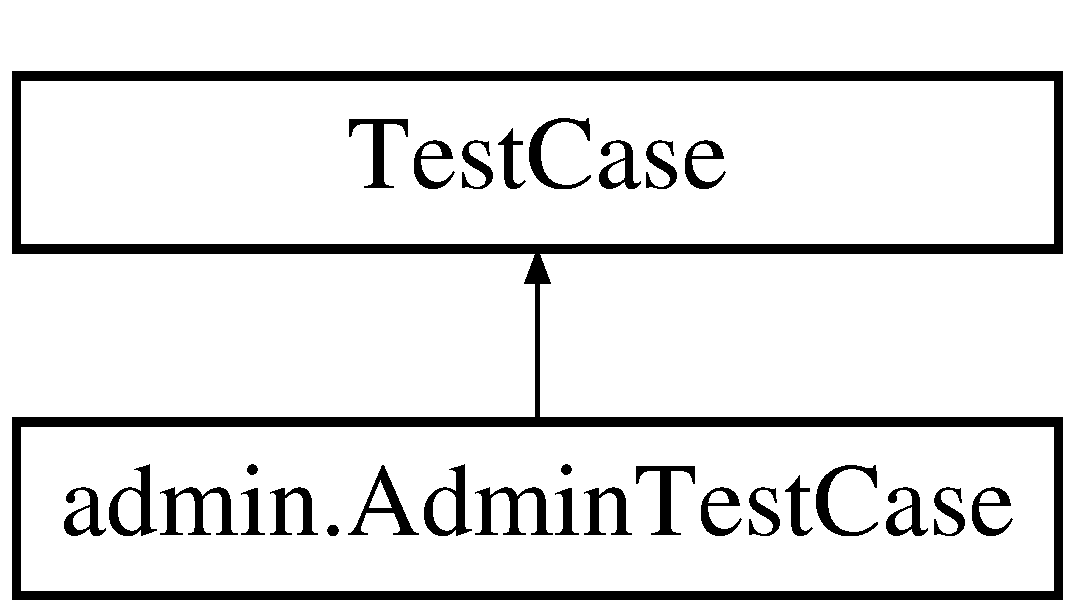
\includegraphics[height=2.000000cm]{de/d4d/classadmin_1_1AdminTestCase}
\end{center}
\end{figure}
\subsection*{Public Member Functions}
\begin{DoxyCompactItemize}
\item 
def \hyperlink{classadmin_1_1AdminTestCase_aca4bb6a593abafd54beab84d0bbdc022}{set\-Up}
\item 
def \hyperlink{classadmin_1_1AdminTestCase_af75fd183f956c48df406d47885d97d7d}{tear\-Down}
\item 
def \hyperlink{classadmin_1_1AdminTestCase_a709452e65fce450953b25bdf40fcc732}{test\-\_\-update\-\_\-seq\-\_\-type}
\item 
def \hyperlink{classadmin_1_1AdminTestCase_a85c52730e0f3491e3b2866404859c6e3}{test\-\_\-decode\-\_\-version}
\item 
def \hyperlink{classadmin_1_1AdminTestCase_a7b416cbb45f1f3a5caaa786979ad0e30}{test\-\_\-match\-\_\-version}
\item 
def \hyperlink{classadmin_1_1AdminTestCase_aeec54ed9163aff1e0615764d4ff2f319}{test\-\_\-read\-\_\-lines}
\end{DoxyCompactItemize}
\subsection*{Public Attributes}
\begin{DoxyCompactItemize}
\item 
\hyperlink{classadmin_1_1AdminTestCase_a235ad774d40bba3600cf09b79dc9f209}{version\-\_\-info}
\item 
\hyperlink{classadmin_1_1AdminTestCase_a6b12aab33be61651698f4b8810678168}{version\-\_\-prefix}
\end{DoxyCompactItemize}


\subsection{Detailed Description}
\begin{DoxyVerb}Test Case of Admin.
\end{DoxyVerb}
 

Definition at line 226 of file \-\_\-\-\_\-init\-\_\-\-\_\-.\-py.



\subsection{Member Function Documentation}
\hypertarget{classadmin_1_1AdminTestCase_aca4bb6a593abafd54beab84d0bbdc022}{\index{admin\-::\-Admin\-Test\-Case@{admin\-::\-Admin\-Test\-Case}!set\-Up@{set\-Up}}
\index{set\-Up@{set\-Up}!admin::AdminTestCase@{admin\-::\-Admin\-Test\-Case}}
\subsubsection[{set\-Up}]{\setlength{\rightskip}{0pt plus 5cm}def admin.\-Admin\-Test\-Case.\-set\-Up (
\begin{DoxyParamCaption}
\item[{}]{self}
\end{DoxyParamCaption}
)}}\label{classadmin_1_1AdminTestCase_aca4bb6a593abafd54beab84d0bbdc022}


Definition at line 229 of file \-\_\-\-\_\-init\-\_\-\-\_\-.\-py.

\hypertarget{classadmin_1_1AdminTestCase_af75fd183f956c48df406d47885d97d7d}{\index{admin\-::\-Admin\-Test\-Case@{admin\-::\-Admin\-Test\-Case}!tear\-Down@{tear\-Down}}
\index{tear\-Down@{tear\-Down}!admin::AdminTestCase@{admin\-::\-Admin\-Test\-Case}}
\subsubsection[{tear\-Down}]{\setlength{\rightskip}{0pt plus 5cm}def admin.\-Admin\-Test\-Case.\-tear\-Down (
\begin{DoxyParamCaption}
\item[{}]{self}
\end{DoxyParamCaption}
)}}\label{classadmin_1_1AdminTestCase_af75fd183f956c48df406d47885d97d7d}


Definition at line 234 of file \-\_\-\-\_\-init\-\_\-\-\_\-.\-py.

\hypertarget{classadmin_1_1AdminTestCase_a85c52730e0f3491e3b2866404859c6e3}{\index{admin\-::\-Admin\-Test\-Case@{admin\-::\-Admin\-Test\-Case}!test\-\_\-decode\-\_\-version@{test\-\_\-decode\-\_\-version}}
\index{test\-\_\-decode\-\_\-version@{test\-\_\-decode\-\_\-version}!admin::AdminTestCase@{admin\-::\-Admin\-Test\-Case}}
\subsubsection[{test\-\_\-decode\-\_\-version}]{\setlength{\rightskip}{0pt plus 5cm}def admin.\-Admin\-Test\-Case.\-test\-\_\-decode\-\_\-version (
\begin{DoxyParamCaption}
\item[{}]{self}
\end{DoxyParamCaption}
)}}\label{classadmin_1_1AdminTestCase_a85c52730e0f3491e3b2866404859c6e3}


Definition at line 245 of file \-\_\-\-\_\-init\-\_\-\-\_\-.\-py.

\hypertarget{classadmin_1_1AdminTestCase_a7b416cbb45f1f3a5caaa786979ad0e30}{\index{admin\-::\-Admin\-Test\-Case@{admin\-::\-Admin\-Test\-Case}!test\-\_\-match\-\_\-version@{test\-\_\-match\-\_\-version}}
\index{test\-\_\-match\-\_\-version@{test\-\_\-match\-\_\-version}!admin::AdminTestCase@{admin\-::\-Admin\-Test\-Case}}
\subsubsection[{test\-\_\-match\-\_\-version}]{\setlength{\rightskip}{0pt plus 5cm}def admin.\-Admin\-Test\-Case.\-test\-\_\-match\-\_\-version (
\begin{DoxyParamCaption}
\item[{}]{self}
\end{DoxyParamCaption}
)}}\label{classadmin_1_1AdminTestCase_a7b416cbb45f1f3a5caaa786979ad0e30}


Definition at line 253 of file \-\_\-\-\_\-init\-\_\-\-\_\-.\-py.

\hypertarget{classadmin_1_1AdminTestCase_aeec54ed9163aff1e0615764d4ff2f319}{\index{admin\-::\-Admin\-Test\-Case@{admin\-::\-Admin\-Test\-Case}!test\-\_\-read\-\_\-lines@{test\-\_\-read\-\_\-lines}}
\index{test\-\_\-read\-\_\-lines@{test\-\_\-read\-\_\-lines}!admin::AdminTestCase@{admin\-::\-Admin\-Test\-Case}}
\subsubsection[{test\-\_\-read\-\_\-lines}]{\setlength{\rightskip}{0pt plus 5cm}def admin.\-Admin\-Test\-Case.\-test\-\_\-read\-\_\-lines (
\begin{DoxyParamCaption}
\item[{}]{self}
\end{DoxyParamCaption}
)}}\label{classadmin_1_1AdminTestCase_aeec54ed9163aff1e0615764d4ff2f319}


Definition at line 276 of file \-\_\-\-\_\-init\-\_\-\-\_\-.\-py.

\hypertarget{classadmin_1_1AdminTestCase_a709452e65fce450953b25bdf40fcc732}{\index{admin\-::\-Admin\-Test\-Case@{admin\-::\-Admin\-Test\-Case}!test\-\_\-update\-\_\-seq\-\_\-type@{test\-\_\-update\-\_\-seq\-\_\-type}}
\index{test\-\_\-update\-\_\-seq\-\_\-type@{test\-\_\-update\-\_\-seq\-\_\-type}!admin::AdminTestCase@{admin\-::\-Admin\-Test\-Case}}
\subsubsection[{test\-\_\-update\-\_\-seq\-\_\-type}]{\setlength{\rightskip}{0pt plus 5cm}def admin.\-Admin\-Test\-Case.\-test\-\_\-update\-\_\-seq\-\_\-type (
\begin{DoxyParamCaption}
\item[{}]{self}
\end{DoxyParamCaption}
)}}\label{classadmin_1_1AdminTestCase_a709452e65fce450953b25bdf40fcc732}


Definition at line 238 of file \-\_\-\-\_\-init\-\_\-\-\_\-.\-py.



\subsection{Member Data Documentation}
\hypertarget{classadmin_1_1AdminTestCase_a235ad774d40bba3600cf09b79dc9f209}{\index{admin\-::\-Admin\-Test\-Case@{admin\-::\-Admin\-Test\-Case}!version\-\_\-info@{version\-\_\-info}}
\index{version\-\_\-info@{version\-\_\-info}!admin::AdminTestCase@{admin\-::\-Admin\-Test\-Case}}
\subsubsection[{version\-\_\-info}]{\setlength{\rightskip}{0pt plus 5cm}admin.\-Admin\-Test\-Case.\-version\-\_\-info}}\label{classadmin_1_1AdminTestCase_a235ad774d40bba3600cf09b79dc9f209}


Definition at line 230 of file \-\_\-\-\_\-init\-\_\-\-\_\-.\-py.

\hypertarget{classadmin_1_1AdminTestCase_a6b12aab33be61651698f4b8810678168}{\index{admin\-::\-Admin\-Test\-Case@{admin\-::\-Admin\-Test\-Case}!version\-\_\-prefix@{version\-\_\-prefix}}
\index{version\-\_\-prefix@{version\-\_\-prefix}!admin::AdminTestCase@{admin\-::\-Admin\-Test\-Case}}
\subsubsection[{version\-\_\-prefix}]{\setlength{\rightskip}{0pt plus 5cm}admin.\-Admin\-Test\-Case.\-version\-\_\-prefix}}\label{classadmin_1_1AdminTestCase_a6b12aab33be61651698f4b8810678168}


Definition at line 231 of file \-\_\-\-\_\-init\-\_\-\-\_\-.\-py.



The documentation for this class was generated from the following file\-:\begin{DoxyCompactItemize}
\item 
admin/\hyperlink{____init_____8py}{\-\_\-\-\_\-init\-\_\-\-\_\-.\-py}\end{DoxyCompactItemize}

\hypertarget{classadmin_1_1ConfigFile}{\section{admin.\-Config\-File Class Reference}
\label{classadmin_1_1ConfigFile}\index{admin.\-Config\-File@{admin.\-Config\-File}}
}


Configuration file.  


Inheritance diagram for admin.\-Config\-File\-:\begin{figure}[H]
\begin{center}
\leavevmode
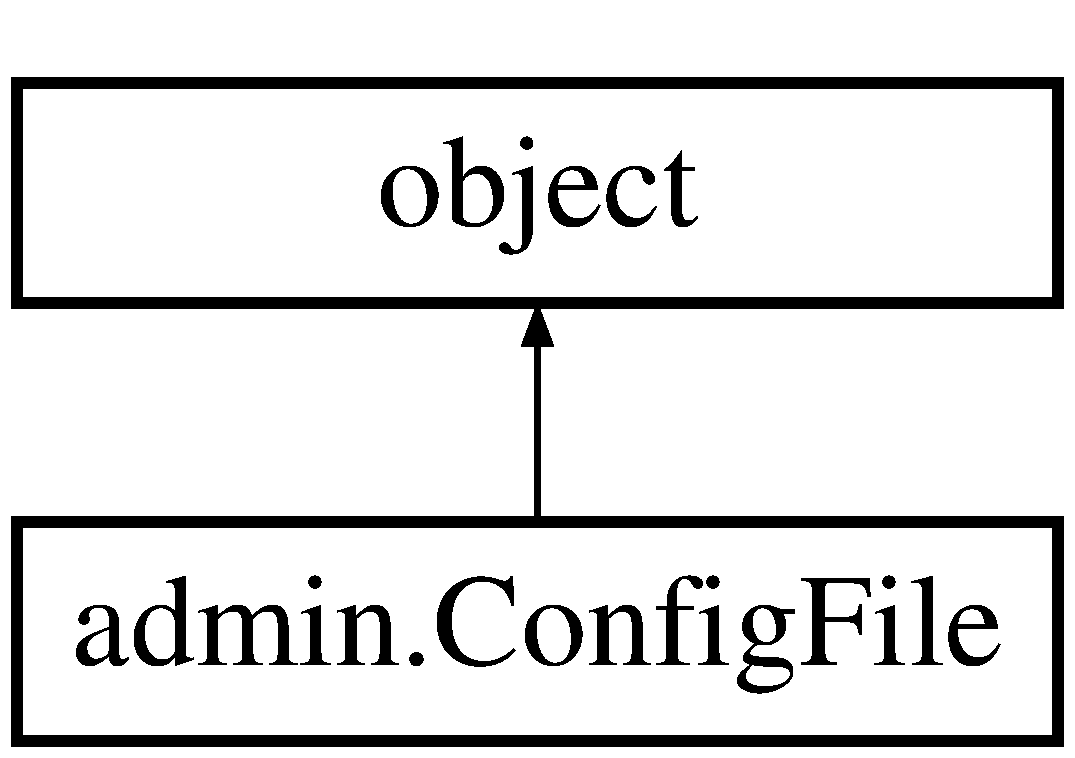
\includegraphics[height=2.000000cm]{d0/d8b/classadmin_1_1ConfigFile}
\end{center}
\end{figure}
\subsection*{Public Member Functions}
\begin{DoxyCompactItemize}
\item 
def \hyperlink{classadmin_1_1ConfigFile_a01f801b702c4cb7e322a8dee7943f5ff}{\-\_\-\-\_\-init\-\_\-\-\_\-}
\begin{DoxyCompactList}\small\item\em Parse configuration file. \end{DoxyCompactList}\item 
def \hyperlink{classadmin_1_1ConfigFile_a3a60d1611c929d782773d73d339454ab}{get}
\begin{DoxyCompactList}\small\item\em Get value of specific option. \end{DoxyCompactList}\item 
def \hyperlink{classadmin_1_1ConfigFile_a05413f3b3760fe95cf8038c400cb2b4f}{set}
\begin{DoxyCompactList}\small\item\em Set value of specific option. \end{DoxyCompactList}\end{DoxyCompactItemize}
\subsection*{Private Attributes}
\begin{DoxyCompactItemize}
\item 
\hyperlink{classadmin_1_1ConfigFile_ada03146a25635d360b9994efcd3eb6ce}{\-\_\-config\-\_\-file}
\item 
\hyperlink{classadmin_1_1ConfigFile_a3f7db562c59049e6a3b28b1fdfafa63e}{\-\_\-sep}
\item 
\hyperlink{classadmin_1_1ConfigFile_ac15829b16933412a7db88d3dacdcf345}{\-\_\-comments}
\item 
\hyperlink{classadmin_1_1ConfigFile_a5a5c415d13ee87e1a03c9f64231a4fc9}{\-\_\-config}
\end{DoxyCompactItemize}


\subsection{Detailed Description}
Configuration file. 

\subsubsection*{Usage}


\begin{DoxyPre}{\ttfamily 
     import os
     import admin}\end{DoxyPre}



\begin{DoxyPre}{\ttfamily      configs = \{'PROJECT\_NAME': '"AAA"',
           'PROJECT\_NUMBER': '1.2.3'\}
     try:
         with open(os.path.join(os.getcwd(), 'Doxyfile'), 'r+') as f:
             config\_file = \hyperlink{classadmin_1_1ConfigFile}{admin.ConfigFile(f)}
             config\_file.set(configs)
         except IOError as e:
             \hyperlink{namespaceadmin_ae1e80d1a965f6551fa95ff379ba2b0cd}{admin.error}('error') 
}\end{DoxyPre}


Definition at line 169 of file \-\_\-\-\_\-init\-\_\-\-\_\-.\-py.



\subsection{Constructor \& Destructor Documentation}
\hypertarget{classadmin_1_1ConfigFile_a01f801b702c4cb7e322a8dee7943f5ff}{\index{admin\-::\-Config\-File@{admin\-::\-Config\-File}!\-\_\-\-\_\-init\-\_\-\-\_\-@{\-\_\-\-\_\-init\-\_\-\-\_\-}}
\index{\-\_\-\-\_\-init\-\_\-\-\_\-@{\-\_\-\-\_\-init\-\_\-\-\_\-}!admin::ConfigFile@{admin\-::\-Config\-File}}
\subsubsection[{\-\_\-\-\_\-init\-\_\-\-\_\-}]{\setlength{\rightskip}{0pt plus 5cm}def admin.\-Config\-File.\-\_\-\-\_\-init\-\_\-\-\_\- (
\begin{DoxyParamCaption}
\item[{}]{self, }
\item[{}]{config\-\_\-file, }
\item[{}]{sep = {\ttfamily '='}, }
\item[{}]{comments = {\ttfamily '\#'}}
\end{DoxyParamCaption}
)}}\label{classadmin_1_1ConfigFile_a01f801b702c4cb7e322a8dee7943f5ff}


Parse configuration file. 


\begin{DoxyParams}{Parameters}
{\em config\-\_\-file} & configuration file object \\
\hline
{\em sep} & separator for option/value pair \\
\hline
{\em comments} & comments leading character \\
\hline
\end{DoxyParams}


Definition at line 175 of file \-\_\-\-\_\-init\-\_\-\-\_\-.\-py.



\subsection{Member Function Documentation}
\hypertarget{classadmin_1_1ConfigFile_a3a60d1611c929d782773d73d339454ab}{\index{admin\-::\-Config\-File@{admin\-::\-Config\-File}!get@{get}}
\index{get@{get}!admin::ConfigFile@{admin\-::\-Config\-File}}
\subsubsection[{get}]{\setlength{\rightskip}{0pt plus 5cm}def admin.\-Config\-File.\-get (
\begin{DoxyParamCaption}
\item[{}]{self, }
\item[{}]{option}
\end{DoxyParamCaption}
)}}\label{classadmin_1_1ConfigFile_a3a60d1611c929d782773d73d339454ab}


Get value of specific option. 


\begin{DoxyParams}{Parameters}
{\em option} & option name \\
\hline
\end{DoxyParams}
\begin{DoxyReturn}{Returns}
option value 
\end{DoxyReturn}

\begin{DoxyExceptions}{Exceptions}
{\em Key\-Error} & -\/ no optinon exists \\
\hline
\end{DoxyExceptions}


Definition at line 195 of file \-\_\-\-\_\-init\-\_\-\-\_\-.\-py.

\hypertarget{classadmin_1_1ConfigFile_a05413f3b3760fe95cf8038c400cb2b4f}{\index{admin\-::\-Config\-File@{admin\-::\-Config\-File}!set@{set}}
\index{set@{set}!admin::ConfigFile@{admin\-::\-Config\-File}}
\subsubsection[{set}]{\setlength{\rightskip}{0pt plus 5cm}def admin.\-Config\-File.\-set (
\begin{DoxyParamCaption}
\item[{}]{self, }
\item[{}]{pairs}
\end{DoxyParamCaption}
)}}\label{classadmin_1_1ConfigFile_a05413f3b3760fe95cf8038c400cb2b4f}


Set value of specific option. 


\begin{DoxyParams}{Parameters}
{\em pairs} & Pairs of option name-\/value. \\
\hline
\end{DoxyParams}


Definition at line 202 of file \-\_\-\-\_\-init\-\_\-\-\_\-.\-py.



\subsection{Member Data Documentation}
\hypertarget{classadmin_1_1ConfigFile_ac15829b16933412a7db88d3dacdcf345}{\index{admin\-::\-Config\-File@{admin\-::\-Config\-File}!\-\_\-comments@{\-\_\-comments}}
\index{\-\_\-comments@{\-\_\-comments}!admin::ConfigFile@{admin\-::\-Config\-File}}
\subsubsection[{\-\_\-comments}]{\setlength{\rightskip}{0pt plus 5cm}admin.\-Config\-File.\-\_\-comments\hspace{0.3cm}{\ttfamily [private]}}}\label{classadmin_1_1ConfigFile_ac15829b16933412a7db88d3dacdcf345}


Definition at line 178 of file \-\_\-\-\_\-init\-\_\-\-\_\-.\-py.

\hypertarget{classadmin_1_1ConfigFile_a5a5c415d13ee87e1a03c9f64231a4fc9}{\index{admin\-::\-Config\-File@{admin\-::\-Config\-File}!\-\_\-config@{\-\_\-config}}
\index{\-\_\-config@{\-\_\-config}!admin::ConfigFile@{admin\-::\-Config\-File}}
\subsubsection[{\-\_\-config}]{\setlength{\rightskip}{0pt plus 5cm}admin.\-Config\-File.\-\_\-config\hspace{0.3cm}{\ttfamily [private]}}}\label{classadmin_1_1ConfigFile_a5a5c415d13ee87e1a03c9f64231a4fc9}


Definition at line 179 of file \-\_\-\-\_\-init\-\_\-\-\_\-.\-py.

\hypertarget{classadmin_1_1ConfigFile_ada03146a25635d360b9994efcd3eb6ce}{\index{admin\-::\-Config\-File@{admin\-::\-Config\-File}!\-\_\-config\-\_\-file@{\-\_\-config\-\_\-file}}
\index{\-\_\-config\-\_\-file@{\-\_\-config\-\_\-file}!admin::ConfigFile@{admin\-::\-Config\-File}}
\subsubsection[{\-\_\-config\-\_\-file}]{\setlength{\rightskip}{0pt plus 5cm}admin.\-Config\-File.\-\_\-config\-\_\-file\hspace{0.3cm}{\ttfamily [private]}}}\label{classadmin_1_1ConfigFile_ada03146a25635d360b9994efcd3eb6ce}


Definition at line 176 of file \-\_\-\-\_\-init\-\_\-\-\_\-.\-py.

\hypertarget{classadmin_1_1ConfigFile_a3f7db562c59049e6a3b28b1fdfafa63e}{\index{admin\-::\-Config\-File@{admin\-::\-Config\-File}!\-\_\-sep@{\-\_\-sep}}
\index{\-\_\-sep@{\-\_\-sep}!admin::ConfigFile@{admin\-::\-Config\-File}}
\subsubsection[{\-\_\-sep}]{\setlength{\rightskip}{0pt plus 5cm}admin.\-Config\-File.\-\_\-sep\hspace{0.3cm}{\ttfamily [private]}}}\label{classadmin_1_1ConfigFile_a3f7db562c59049e6a3b28b1fdfafa63e}


Definition at line 177 of file \-\_\-\-\_\-init\-\_\-\-\_\-.\-py.



The documentation for this class was generated from the following file\-:\begin{DoxyCompactItemize}
\item 
admin/\hyperlink{____init_____8py}{\-\_\-\-\_\-init\-\_\-\-\_\-.\-py}\end{DoxyCompactItemize}

\hypertarget{classadmin_1_1project_1_1Project}{\section{admin.\-project.\-Project Class Reference}
\label{classadmin_1_1project_1_1Project}\index{admin.\-project.\-Project@{admin.\-project.\-Project}}
}


\hyperlink{classadmin_1_1project_1_1Project}{Project}.  


Inheritance diagram for admin.\-project.\-Project\-:\begin{figure}[H]
\begin{center}
\leavevmode
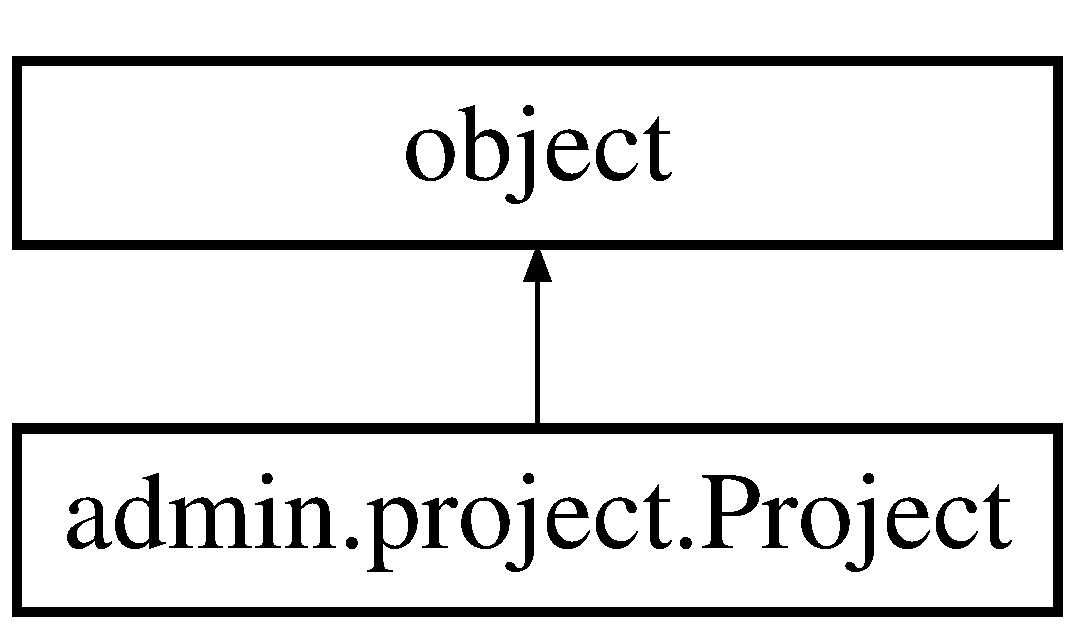
\includegraphics[height=2.000000cm]{d0/d08/classadmin_1_1project_1_1Project}
\end{center}
\end{figure}
\subsection*{Public Member Functions}
\begin{DoxyCompactItemize}
\item 
def \hyperlink{classadmin_1_1project_1_1Project_aeb44db1aabe1eae8b7d970702270dc61}{\-\_\-\-\_\-init\-\_\-\-\_\-}
\begin{DoxyCompactList}\small\item\em Create an instance of \hyperlink{classadmin_1_1project_1_1Project}{Project}. \end{DoxyCompactList}\item 
def \hyperlink{classadmin_1_1project_1_1Project_a83f54c8b5d69acab088d1cc1e6e52901}{uwsgi}
\item 
def \hyperlink{classadmin_1_1project_1_1Project_a288339834e2636bf372f02030808d2ac}{django}
\item 
def \hyperlink{classadmin_1_1project_1_1Project_af8f058021d27f5d4f5c226afb10b4ada}{doxygen}
\begin{DoxyCompactList}\small\item\em Generate documentation for codes under Git by Doxygen. \end{DoxyCompactList}\end{DoxyCompactItemize}
\subsection*{Public Attributes}
\begin{DoxyCompactItemize}
\item 
\hyperlink{classadmin_1_1project_1_1Project_add0eb047a815df47b9b888aa8a028b77}{lang}
\item 
\hyperlink{classadmin_1_1project_1_1Project_a4a925408cb4575a4f8e880918decdf7d}{path}
\item 
\hyperlink{classadmin_1_1project_1_1Project_a9b8c34b91f1ecdbbdcfea42e771dd6d6}{name}
\item 
\hyperlink{classadmin_1_1project_1_1Project_ac3e2b73e80631fe2171b8d4b236f2e53}{brief}
\item 
\hyperlink{classadmin_1_1project_1_1Project_aead4e47be18c6ddbfd19d3b5aab88bda}{version\-\_\-info}
\end{DoxyCompactItemize}
\subsection*{Private Attributes}
\begin{DoxyCompactItemize}
\item 
\hyperlink{classadmin_1_1project_1_1Project_a9357a34aaccfd3fc391b4081f6794ee8}{\-\_\-build\-\_\-dir}
\end{DoxyCompactItemize}


\subsection{Detailed Description}
\hyperlink{classadmin_1_1project_1_1Project}{Project}. 

\subsubsection*{Usage}


\begin{DoxyPre}{\ttfamily 
      import admin
      import \hyperlink{namespaceadmin_1_1project}{admin.project}}\end{DoxyPre}



\begin{DoxyPre}{\ttfamily       proj = \hyperlink{classadmin_1_1project_1_1Project}{admin.project.Project}(lang=['python'])
      try:
          \# Setup uWSGI server
          proj.uwsgi()}\end{DoxyPre}



\begin{DoxyPre}{\ttfamily           \# Setup Django
          proj.django()}\end{DoxyPre}



\begin{DoxyPre}{\ttfamily           \# Generate documentation
          proj.doxygen()
      except subprocess.CalledProcessError as e:
          \hyperlink{namespaceadmin_ae1e80d1a965f6551fa95ff379ba2b0cd}{admin.error}('error')
      except IOError as e:
          \hyperlink{namespaceadmin_ae1e80d1a965f6551fa95ff379ba2b0cd}{admin.error}('error')
  }\end{DoxyPre}
 

Definition at line 56 of file project.\-py.



\subsection{Constructor \& Destructor Documentation}
\hypertarget{classadmin_1_1project_1_1Project_aeb44db1aabe1eae8b7d970702270dc61}{\index{admin\-::project\-::\-Project@{admin\-::project\-::\-Project}!\-\_\-\-\_\-init\-\_\-\-\_\-@{\-\_\-\-\_\-init\-\_\-\-\_\-}}
\index{\-\_\-\-\_\-init\-\_\-\-\_\-@{\-\_\-\-\_\-init\-\_\-\-\_\-}!admin::project::Project@{admin\-::project\-::\-Project}}
\subsubsection[{\-\_\-\-\_\-init\-\_\-\-\_\-}]{\setlength{\rightskip}{0pt plus 5cm}def admin.\-project.\-Project.\-\_\-\-\_\-init\-\_\-\-\_\- (
\begin{DoxyParamCaption}
\item[{}]{self, }
\item[{}]{lang, }
\item[{}]{build\-\_\-dir = {\ttfamily 'build'}, }
\item[{}]{default\-\_\-version = {\ttfamily '0.0.0'}}
\end{DoxyParamCaption}
)}}\label{classadmin_1_1project_1_1Project_aeb44db1aabe1eae8b7d970702270dc61}


Create an instance of \hyperlink{classadmin_1_1project_1_1Project}{Project}. 


\begin{DoxyParams}{Parameters}
{\em lang} & programming language (python, c, java, cpp) \\
\hline
{\em build\-\_\-dir} & building directory \\
\hline
{\em default\-\_\-version} & default version string \\
\hline
\end{DoxyParams}


Definition at line 62 of file project.\-py.



\subsection{Member Function Documentation}
\hypertarget{classadmin_1_1project_1_1Project_a288339834e2636bf372f02030808d2ac}{\index{admin\-::project\-::\-Project@{admin\-::project\-::\-Project}!django@{django}}
\index{django@{django}!admin::project::Project@{admin\-::project\-::\-Project}}
\subsubsection[{django}]{\setlength{\rightskip}{0pt plus 5cm}def admin.\-project.\-Project.\-django (
\begin{DoxyParamCaption}
\item[{}]{self, }
\item[{}]{site = {\ttfamily 'mysite'}, }
\item[{}]{nginx = {\ttfamily None}, }
\item[{}]{run = {\ttfamily False}}
\end{DoxyParamCaption}
)}}\label{classadmin_1_1project_1_1Project_a288339834e2636bf372f02030808d2ac}


Definition at line 150 of file project.\-py.

\hypertarget{classadmin_1_1project_1_1Project_af8f058021d27f5d4f5c226afb10b4ada}{\index{admin\-::project\-::\-Project@{admin\-::project\-::\-Project}!doxygen@{doxygen}}
\index{doxygen@{doxygen}!admin::project::Project@{admin\-::project\-::\-Project}}
\subsubsection[{doxygen}]{\setlength{\rightskip}{0pt plus 5cm}def admin.\-project.\-Project.\-doxygen (
\begin{DoxyParamCaption}
\item[{}]{self, }
\item[{}]{doxyfile = {\ttfamily 'Doxyfile'}}
\end{DoxyParamCaption}
)}}\label{classadmin_1_1project_1_1Project_af8f058021d27f5d4f5c226afb10b4ada}


Generate documentation for codes under Git by Doxygen. 


\begin{DoxyParams}{Parameters}
{\em doxyfile} & name of Doxygen configuration file \\
\hline
\end{DoxyParams}

\begin{DoxyExceptions}{Exceptions}
{\em subprocess.\-Called\-Process\-Error} & -\/ from {\ttfamily doxygen} \\
\hline
{\em I\-O\-Error} & -\/ configuration file written error \\
\hline
\end{DoxyExceptions}


Definition at line 174 of file project.\-py.

\hypertarget{classadmin_1_1project_1_1Project_a83f54c8b5d69acab088d1cc1e6e52901}{\index{admin\-::project\-::\-Project@{admin\-::project\-::\-Project}!uwsgi@{uwsgi}}
\index{uwsgi@{uwsgi}!admin::project::Project@{admin\-::project\-::\-Project}}
\subsubsection[{uwsgi}]{\setlength{\rightskip}{0pt plus 5cm}def admin.\-project.\-Project.\-uwsgi (
\begin{DoxyParamCaption}
\item[{}]{self, }
\item[{}]{wsgi\-\_\-file = {\ttfamily '\-\_\-setup/uwsgi\-\_\-app.py'}, }
\item[{}]{django = {\ttfamily None}, }
\item[{}]{nginx = {\ttfamily None}, }
\item[{}]{run = {\ttfamily False}}
\end{DoxyParamCaption}
)}}\label{classadmin_1_1project_1_1Project_a83f54c8b5d69acab088d1cc1e6e52901}


Definition at line 104 of file project.\-py.



\subsection{Member Data Documentation}
\hypertarget{classadmin_1_1project_1_1Project_a9357a34aaccfd3fc391b4081f6794ee8}{\index{admin\-::project\-::\-Project@{admin\-::project\-::\-Project}!\-\_\-build\-\_\-dir@{\-\_\-build\-\_\-dir}}
\index{\-\_\-build\-\_\-dir@{\-\_\-build\-\_\-dir}!admin::project::Project@{admin\-::project\-::\-Project}}
\subsubsection[{\-\_\-build\-\_\-dir}]{\setlength{\rightskip}{0pt plus 5cm}admin.\-project.\-Project.\-\_\-build\-\_\-dir\hspace{0.3cm}{\ttfamily [private]}}}\label{classadmin_1_1project_1_1Project_a9357a34aaccfd3fc391b4081f6794ee8}


Definition at line 66 of file project.\-py.

\hypertarget{classadmin_1_1project_1_1Project_ac3e2b73e80631fe2171b8d4b236f2e53}{\index{admin\-::project\-::\-Project@{admin\-::project\-::\-Project}!brief@{brief}}
\index{brief@{brief}!admin::project::Project@{admin\-::project\-::\-Project}}
\subsubsection[{brief}]{\setlength{\rightskip}{0pt plus 5cm}admin.\-project.\-Project.\-brief}}\label{classadmin_1_1project_1_1Project_ac3e2b73e80631fe2171b8d4b236f2e53}


Definition at line 70 of file project.\-py.

\hypertarget{classadmin_1_1project_1_1Project_add0eb047a815df47b9b888aa8a028b77}{\index{admin\-::project\-::\-Project@{admin\-::project\-::\-Project}!lang@{lang}}
\index{lang@{lang}!admin::project::Project@{admin\-::project\-::\-Project}}
\subsubsection[{lang}]{\setlength{\rightskip}{0pt plus 5cm}admin.\-project.\-Project.\-lang}}\label{classadmin_1_1project_1_1Project_add0eb047a815df47b9b888aa8a028b77}


Definition at line 63 of file project.\-py.

\hypertarget{classadmin_1_1project_1_1Project_a9b8c34b91f1ecdbbdcfea42e771dd6d6}{\index{admin\-::project\-::\-Project@{admin\-::project\-::\-Project}!name@{name}}
\index{name@{name}!admin::project::Project@{admin\-::project\-::\-Project}}
\subsubsection[{name}]{\setlength{\rightskip}{0pt plus 5cm}admin.\-project.\-Project.\-name}}\label{classadmin_1_1project_1_1Project_a9b8c34b91f1ecdbbdcfea42e771dd6d6}


Definition at line 65 of file project.\-py.

\hypertarget{classadmin_1_1project_1_1Project_a4a925408cb4575a4f8e880918decdf7d}{\index{admin\-::project\-::\-Project@{admin\-::project\-::\-Project}!path@{path}}
\index{path@{path}!admin::project::Project@{admin\-::project\-::\-Project}}
\subsubsection[{path}]{\setlength{\rightskip}{0pt plus 5cm}admin.\-project.\-Project.\-path}}\label{classadmin_1_1project_1_1Project_a4a925408cb4575a4f8e880918decdf7d}


Definition at line 64 of file project.\-py.

\hypertarget{classadmin_1_1project_1_1Project_aead4e47be18c6ddbfd19d3b5aab88bda}{\index{admin\-::project\-::\-Project@{admin\-::project\-::\-Project}!version\-\_\-info@{version\-\_\-info}}
\index{version\-\_\-info@{version\-\_\-info}!admin::project::Project@{admin\-::project\-::\-Project}}
\subsubsection[{version\-\_\-info}]{\setlength{\rightskip}{0pt plus 5cm}admin.\-project.\-Project.\-version\-\_\-info}}\label{classadmin_1_1project_1_1Project_aead4e47be18c6ddbfd19d3b5aab88bda}


Definition at line 79 of file project.\-py.



The documentation for this class was generated from the following file\-:\begin{DoxyCompactItemize}
\item 
admin/\hyperlink{project_8py}{project.\-py}\end{DoxyCompactItemize}

\chapter{File Documentation}
\hypertarget{____init_____8py}{\section{admin/\-\_\-\-\_\-init\-\_\-\-\_\-.py File Reference}
\label{____init_____8py}\index{admin/\-\_\-\-\_\-init\-\_\-\-\_\-.\-py@{admin/\-\_\-\-\_\-init\-\_\-\-\_\-.\-py}}
}
\subsection*{Classes}
\begin{DoxyCompactItemize}
\item 
class \hyperlink{classadmin_1_1ConfigFile}{admin.\-Config\-File}
\begin{DoxyCompactList}\small\item\em Configuration file. \end{DoxyCompactList}\item 
class \hyperlink{classadmin_1_1AdminTestCase}{admin.\-Admin\-Test\-Case}
\end{DoxyCompactItemize}
\subsection*{Namespaces}
\begin{DoxyCompactItemize}
\item 
\hyperlink{namespaceadmin}{admin}
\end{DoxyCompactItemize}
\subsection*{Functions}
\begin{DoxyCompactItemize}
\item 
def \hyperlink{namespaceadmin_ae1e80d1a965f6551fa95ff379ba2b0cd}{admin.\-error}
\begin{DoxyCompactList}\small\item\em Print error messages. \end{DoxyCompactList}\item 
def \hyperlink{namespaceadmin_a575bcc44ebed9e68574ccb636a66a4d2}{admin.\-debug}
\begin{DoxyCompactList}\small\item\em Print debugging message. \end{DoxyCompactList}\item 
def \hyperlink{namespaceadmin_ae1dbeff3e935d67ed99b95eb814c9a11}{admin.\-update\-\_\-seq\-\_\-type}
\begin{DoxyCompactList}\small\item\em Update type of all elements in specific sequence. \end{DoxyCompactList}\item 
def \hyperlink{namespaceadmin_a8b0cb2905f04979a2db7cf3bb181ad00}{admin.\-force\-\_\-remove}
\begin{DoxyCompactList}\small\item\em Command {\ttfamily rm -\/f}. \end{DoxyCompactList}\item 
def \hyperlink{namespaceadmin_a186685a5e2120c71362c46b35f0705c3}{admin.\-eintr\-\_\-retry}
\begin{DoxyCompactList}\small\item\em Restart a system call interrupted by {\ttfamily E\-I\-N\-T\-R}. \end{DoxyCompactList}\item 
def \hyperlink{namespaceadmin_a2605170b60fdae0f26432f209ed71f49}{admin.\-decode\-\_\-version}
\begin{DoxyCompactList}\small\item\em Decode version information string. \end{DoxyCompactList}\item 
def \hyperlink{namespaceadmin_a89c4e2a6cc63b64d27825da9eb414b98}{admin.\-match\-\_\-version}
\begin{DoxyCompactList}\small\item\em Match the specific version. \end{DoxyCompactList}\item 
def \hyperlink{namespaceadmin_ae034627a9fca691b23ee55d255113a81}{admin.\-read\-\_\-lines}
\begin{DoxyCompactList}\small\item\em Read specific line(s) with line number(s). \end{DoxyCompactList}\end{DoxyCompactItemize}
\subsection*{Variables}
\begin{DoxyCompactItemize}
\item 
tuple \hyperlink{namespaceadmin_acbbc1dce90a9452383bd52c69b4a7489}{admin.\-Version} = namedtuple('Version', 'major, minor, patch')
\end{DoxyCompactItemize}

\hypertarget{project_8py}{\section{/home/ly/admin-\/linux/admin/project.py File Reference}
\label{project_8py}\index{/home/ly/admin-\/linux/admin/project.\-py@{/home/ly/admin-\/linux/admin/project.\-py}}
}
\subsection*{Classes}
\begin{DoxyCompactItemize}
\item 
class \hyperlink{classadmin_1_1project_1_1Project}{admin.\-project.\-Project}
\begin{DoxyCompactList}\small\item\em \hyperlink{classadmin_1_1project_1_1Project}{Project}. \end{DoxyCompactList}\end{DoxyCompactItemize}
\subsection*{Namespaces}
\begin{DoxyCompactItemize}
\item 
\hyperlink{namespaceadmin_1_1project}{admin.\-project}
\end{DoxyCompactItemize}

%--- End generated contents ---

% Index
\newpage
\phantomsection
\addcontentsline{toc}{chapter}{Index}
\printindex

\end{document}
